\chapter{Parameter Estimation I: Bayes' Box}
One of the most important times to use Bayes' rule is when you want to do
{\it parameter estimation}. Parameter estimation is a fairly common
situation in statistics. In fact, it is possible to interpret almost any
problem in statistics as a parameter estimation problem and approach it
in this way!

Firstly, what is a parameter? One way to think of a parameter is that
it is just a fancy term for a quantity or a number that is
unknown\footnote{Another use for the term parameter
is any quantity that something else depends on. For example, a normal distribution
has a mean $\mu$ and a standard deviation $\sigma$ that defines which normal
distribution we are talking about. $\mu$ and $\sigma$ are then said to be
parameters of the normal distribution.}.
For example, how many people are currently in New
Zealand? Well, a Google search suggests 4.405 million. But that does not mean
there are {\bf exactly} 4,405,000 people. It could be a bit more or a bit
less. Maybe it is 4,405,323, or maybe it is 4,403,886. We don't really know.
We could call the true number of people in New Zealand right now $\theta$, or
we could use some other letter or symbol if we want. When talking about
parameter estimation in general we often call the unknown parameter(s)
$\theta$, but in specific applications we will call the parameter(s) something
else more appropriate for that application.

The key is to realise that we can use the Bayes' Box, like in previous chapters.
But now, our list of possible hypotheses is a list of possible values for
the unknown parameter. For example, a Bayes' Box for the precise number of
people in New Zealand might look something like the one in
Table~\ref{tab:nz_pop}.

\begin{table}[ht!]
\begin{center}
\begin{tabular}{|c|c|c|c|c|}
\hline
{\bf Possible Hypotheses} & {\tt prior} & {\tt likelihood} &
{\tt prior $\times$ likelihood} & {\tt posterior}\\
\hline
\ldots & \ldots & \ldots & \ldots & \ldots\\
$\theta = 4404999$ & 0.000001 & \ldots   & \ldots  & \ldots\\
$\theta = 4405000$ & 0.000001 & \ldots   & \ldots  & \ldots\\
$\theta = 4405001$ & 0.000001 & \ldots   & \ldots  & \ldots\\
$\theta = 4405002$ & 0.000001 & \ldots   & \ldots  & \ldots\\
$\theta = 4405003$ & 0.000001 & \ldots   & \ldots  & \ldots\\
$\theta = 4405004$ & 0.000001 & \ldots   & \ldots  & \ldots\\
$\theta = 4405005$ & 0.000001 & \ldots   & \ldots  & \ldots\\
$\theta = 4405006$ & 0.000001 & \ldots   & \ldots  & \ldots\\
\ldots & \ldots & \ldots & \ldots & \ldots\\
\hline
Totals: & 1 & & \ldots & 1\\
\hline
\end{tabular}
\caption{\it An example of how a Bayes' Box may be used in a parameter
estimation situation.\label{tab:nz_pop}}
\end{center}
\end{table}

There are a few things to note about this Bayes' box. Firstly, it is big, which
is why I just put a bunch of ``\ldots''s in there instead of making up numbers.
There are lots of possible hypotheses, each one corresponding to a possible value
for
$\theta$. The prior probabilities I have put in the second column were for
illustrative purposes. They needn't necessarily all be equal (although that is
often a convenient assumption). All the
stuff we've seen in smaller examples of Bayes' rule and/or use of a Bayes' Box
still applies here. The likelihoods will
still be calculated by seeing how the probability of the data depends on the
value of the unknown parameter. You still go through all the same steps,
multiplying prior times likelihood and then normalising that to get the
posterior probabilities for all of the possibilities listed. Note that a set
of possible values together with the probabilities is what is commonly termed
a {\it probability distribution}. In basic Bayesian problems, like in the
introductory chapters, we start with some prior probabilities and update them
to get posterior probabilities. In parameter estimation, we start with a prior
{\it distribution} for the unknown parameter(s) and update that to get a
posterior {\it distribution} for the unknown parameter(s).

\begin{framed}
{\bf
A quantity which has a probability associated with each possible value is
traditionally called a ``random variable''. Random variables have probability
distributions associated with them. In Bayesian stats, an unknown
parameter looks mathematically like a ``random variable'', but I try to avoid
the word random itself because it usually has connotations about something that
fluctuates or varies. In Bayesian statistics, the prior distribution and
posterior distribution only describe our uncertainty. The actual parameter is
a single fixed number.}
\end{framed} 

\section{Parameter Estimation: Bus Example}
This is a beginning example of parameter estimation from a Bayesian point of
view. It shows the various features that are always present in a Bayesian
parameter estimation problem. There will be a prior distribution, the likelihood,
and the posterior distribution. We will spend a lot of time on this problem but
keep in mind that this is just a single example, and certain things about this
example (such as the choice of the prior and the likelihood) are specific to
this example only, while other things about it are very general and will apply
in all parameter estimation problems. You will see and gain experience with
different problems in lectures, labs, and assignments.

After moving to Auckland, I decided that I would take the bus to work
each day. However, I wasn't very confident with the bus system in my new city,
so for the first
week I just took the first bus that came along and was heading in the right
direction, towards the city. In the first week, I caught 5 morning buses.
Of these 5 buses, two of them took me to the right place, while three of them
took me far from work, leaving me with an extra 20 minute walk. Given this
information, I would like to try to infer the proportion
of the buses that are ``good'', that would take me right to campus. Let us call
this fraction $\theta$ and we will infer $\theta$ using the Bayesian framework.
We will start with a prior distribution that describes initial uncertainty about
$\theta$ and update this to get the posterior distribution, using the data that
2/5 buses I took were ``good''.

First we must think about the meaning of the parameter $\theta$ in our particular
problem so we can choose a sensible prior distribution. Since $\theta$ is, in
this example, a proportion, we know it cannot be less than 0 or greater than 1.
In principle, $\theta$ could be any real value between 0 and 1. To keep things
simple {\it to begin with}, we shall make an approximation and assume that the
set of possible values for $\theta$ is:
\begin{center}
$\{0, 0.1, 0.2, 0.3, 0.4, 0.5, 0.6, 0.7, 0.8, 0.9, 1\}$.
\end{center}
This discrete
approximation means that we can use a Bayes' Box. The first things to fill out
in the Bayes' Box are the possible values and the prior probabilities (the prior
distribution). For starters, let us assume that before we got the data (two
successes out of 5 trials), we were very uncertain about the value of $\theta$,
and this can be modelled by using a uniform prior distribution. There are 11
possible values for $\theta$ that are being considered with our discrete
approximation, so the probability of each is $1/11 = 0.0909$. The partially
complete Bayes' Box is given in Table~\ref{tab:bus_bayes_box1}. Note the
new notation that I have put in the column titles. We will use this notation
in all of our parameter estimation examples (although the parameter(s) and data
may have different symbols when $\theta$ and $x$ respectively are not
appropriate).

\begin{table}[ht!]
\begin{center}
\begin{tabular}{|c|c|c|c|c|}
\hline
\tt{possible values} & \tt{prior} & \tt{likelihood} & \tt{prior} $\times$ \tt{likelihood} & \tt{posterior}\\
$\theta$ & $p(\theta)$ & $p(x|\theta)$ & $p(\theta)p(x|\theta)$ & $p(\theta|x)$\\
\hline
0 & 0.0909 &  &  & \\
0.1 & 0.0909 &  &  & \\
0.2 & 0.0909 &  &  & \\
0.3 & 0.0909 &  &  & \\
0.4 & 0.0909 &  &  & \\
0.5 & 0.0909 &  &  & \\
0.6 & 0.0909 &  &  & \\
0.7 & 0.0909 &  &  & \\
0.8 & 0.0909 &  &  & \\
0.9 & 0.0909 &  &  & \\
1 & 0.0909 &  &  & \\
\hline
Totals & 1 & & & 1\\
\hline
\end{tabular}
\caption{\it Starting to make a Bayes' Box for the bus problem. This one
just has the possible parameter values and the prior distribution.
\label{tab:bus_bayes_box1}}
\end{center}
\end{table}

To get the likelihoods, we need to think about the properties of our experiment.
In particular, we should imagine that we knew the value of $\theta$ and were
trying to predict what experimental outcome would occur. 
Recall that,
if there are $N$
repetitions of a ``random experiment'' and the ``success'' probability is
$\theta$ at each repitition,
then the number of ``successes'' $x$ has a binomial distribution:
\begin{eqnarray}
p(x|\theta) &=& \left(\begin{array}{c}N \\ x\end{array}\right)
\theta^x\left(1-\theta\right)^{N - x}.\label{eq:binomial_likelihood2}
\end{eqnarray}
where $\left(\begin{array}{c}N \\ x\end{array}\right) = \frac{N!}{x!(N-x)!}$.
This is the probability mass function for $x$ (if we imagine $\theta$ to be known), hence the notation $p(x|\theta)$, read as ``the probability distribution for $x$ given $\theta$''.
Since there are five trials
($N=5$) in the bus problem, the number of successes $x$ must be one of
0, 1, 2, 3, 4, or 5.
If $\theta$ is a high number close to 1, then we would expect the resulting
value of the data (number of successes) $x$ to be something high like 4 or 5. Low values for $x$ would
still be possible but they would have a small probability. If $\theta$ is a
small number, we would expect the data to be 0, 1, or 2, with less probability
for more than 2 successes. This is just saying in words what is written
precisely in Equation~\ref{eq:binomial_likelihood}. The probability distribution
for the data $x$ is plotted in Figure~\ref{fig:binomial} for three illustrative
values of the parameter $\theta$.
\begin{figure}[h!]
\begin{center}
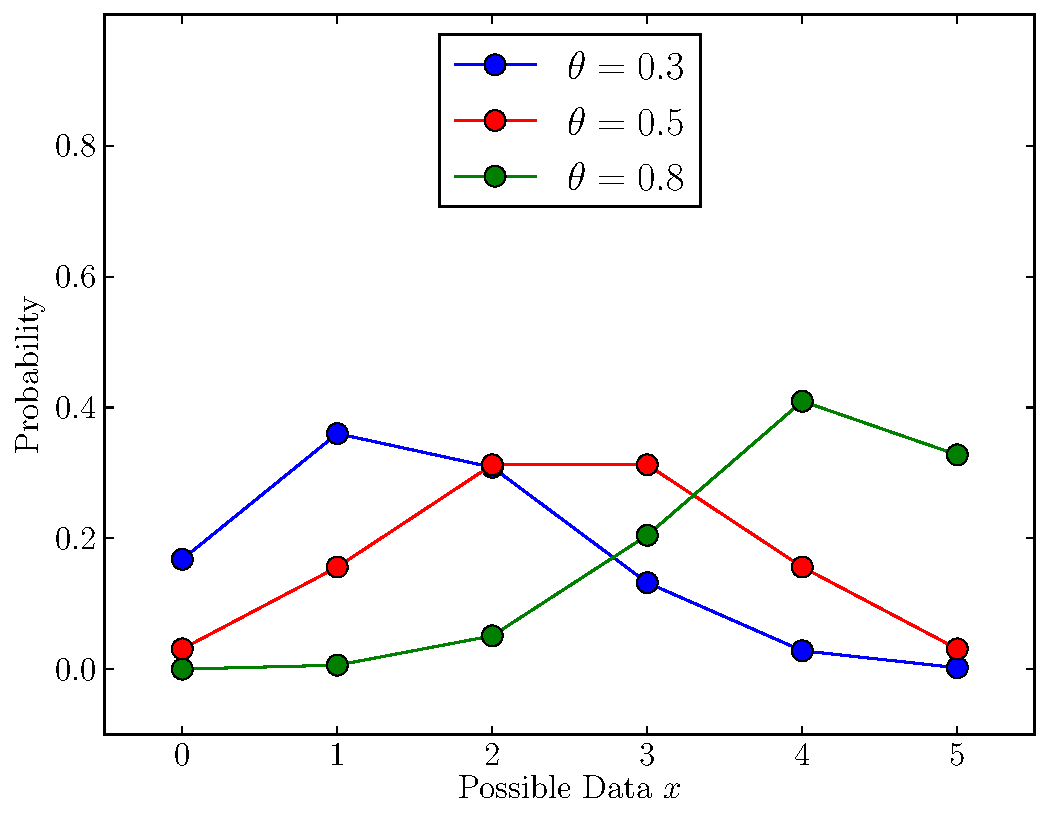
\includegraphics[scale=0.6]{Figures/binomial.pdf}
\caption{\it The binomial likelihood, viewed as a probability distribution for the
data $x$, for three different values of the parameter $\theta$. If $\theta$ is
low then we would expect to see lower values for the data. If $\theta$ is high
then high values are more probable (but all values from 0 to 5 inclusive are
still possible). The actual observed value of the data was $x=2$. If we focus
only on the values of the curves at $x=2$, then the heights of the curves give
the likelihood values for these three illustrative values of $\theta$.
\label{fig:binomial}}
\end{center}
\end{figure}
To obtain the actual likelihood values that go into the Bayes' Box, we can
simply substitute in the known values $N=5$ and $x=2$:
\begin{eqnarray}
P(x=2|\theta) &=& \left(\begin{array}{c}5 \\ 2\end{array}\right)
\theta^2\left(1-\theta\right)^{5 - 2}\\
&=& 10\times\theta^2\left(1-\theta\right)^3.\label{eq:binomial_likelihood3}
\end{eqnarray}
The resulting equation depends on $\theta$ only! We can go through the list of
$\theta$ values and get a numerical answer for the likelihood $P(x=2|\theta)$,
which is what we need for the Bayes' Box. The final steps are, as usual, to
multiply the prior by the likelihood and then normalise that to get the
posterior distribution. The completed Bayes' Box is given in
Table~\ref{tab:bus_bayes_box2}.

\begin{table}[ht!]
\begin{center}
\begin{tabular}{|c|c|c|c|c|}
\hline
\tt{possible values} & \tt{prior} & \tt{likelihood} & \tt{prior} $\times$ \tt{likelihood} & \tt{posterior}\\
$\theta$ & $p(\theta)$ & $p(x|\theta)$ & $p(\theta)p(x|\theta)$ & $p(\theta|x)$\\
\hline
0 & 0.0909 & 0 & 0 & 0\\
0.1 & 0.0909 & 0.0729 & 0.0066 & 0.0437\\
0.2 & 0.0909 & 0.2048 & 0.0186 & 0.1229\\
0.3 & 0.0909 & 0.3087 & 0.0281 & 0.1852\\
0.4 & 0.0909 & 0.3456 & 0.0314 & 0.2074\\
0.5 & 0.0909 & 0.3125 & 0.0284 & 0.1875\\
0.6 & 0.0909 & 0.2304 & 0.0209 & 0.1383\\
0.7 & 0.0909 & 0.1323 & 0.0120 & 0.0794\\
0.8 & 0.0909 & 0.0512 & 0.0047 & 0.0307\\
0.9 & 0.0909 & 0.0081 & 0.0007 & 0.0049\\
1 & 0.0909 & 0 & 0 & 0\\
\hline
Totals & 1 & & 0.1515 & 1\\
\hline
\end{tabular}
\caption{\it The completed Bayes' Box for the bus problem
(using a binomial likelihood).
\label{tab:bus_bayes_box2}}
\end{center}
\end{table}


There are a few interesting values in the likelihood column that should help you
to understand the concept of likelihood a bit better. Look at the likelihood for
$\theta = 0$: it is zero. What does this mean? It means that if we imagine
$\theta=0$ is the true solution, the probability of obtaining the data that we
got ($x=2$ successes) would be zero. That makes sense! If $\theta=0$, it means
none of the buses are the ``good'' buses, so how could I have caught a
good bus twice? The probability of that is zero.

The likelihood for $\theta=1$ is also zero for similar reasons. If all of the
buses are good, then having 2/5 successes is impossible. You would get 5/5
with 100\% certainty. So $P(x=2|\theta=1) = 0$. The likelihood is highest
for $\theta = 0.4$, which just so happens to equal 2/5. This $\theta=0.4$ predicted
the data best. It does
not necessarily mean that $\theta=0.4$ is the most probable value. That depends
on the prior as well (but with a uniform prior, it does end up being that way.
As you can see in the posterior distribution column, $\theta=0.4$ has the
highest probability in this case).

Even though this example is meant to be introductory, there is a subtlety
that has been swept under the rug. Notice that our data consisted of the fact
that we got 2/5 successes in the experiment. When we worked out the likelihood,
we were considering the probability of getting $x=2$, but we didn't have a
probability for $N=5$. In principle, we could treat $x$ and $N$ as two separate data sets.
We could first update from the prior to the posterior given $N=5$, and then update
again to take into account $x$ as well as $N$. However, the first update would
be a bit weird. Why would knowing the number of trials tell you anything about
the success probability? Effectively, what we have done in our analysis is assume that $N=5$ is prior information that lurks in the background the whole time. Therefore our uniform prior for $\theta$ already ``knows''
that $N=5$, so we didn't have to consider $P(N=5|\theta)$ in the likelihood.
This subtlety usually doesn't matter much.

\section{Prediction in the Bus Problem}\label{sec:prediction_bus_problem}
We have now seen how to use information (data) to update from a prior distribution
to a posterior distribution when the set of possible values is discrete. The
posterior distribution is the complete answer to the problem. It tells us exactly
how strongly we should believe in the various possible solutions (possible
values for the unknown parameter). However, there
are other things we might want to do with this information. Predicting the future
is one! It's fun, but risky. Here we will look at how it is done using the Bayesian
framework, continuing with the bus example. To be concrete, we are interested
in the following question: {\it what is the probability that I will catch the
right bus tomorrow?}. This is like trying to predict the result of a future
experiment.

Suppose we knew the true value of $\theta$ was 0.3. Then, we would know
the probability of catching the right bus tomorrow is 0.3. If we knew the
true value of $\theta$ was 0.4, we would say the probability of catching
the right bus tomorrow is 0.4. The problem is, we don't know what the true value
is. We only have the posterior distribution. Luckily, the sum rule of
probability (combined with the product rule) can help us out. We are interested in whether I will get the good
bus tomorrow. There are 11 different ways that can happen. Either $\theta=0$ and
I get the good bus, or $\theta=0.1$ and I get the good bus, or $\theta=0.2$ and
I get the good bus, and so on. These 11 ways are all mutually exclusive. That is,
only one of them can be true (since $\theta$ is actually just a single number).
Mathematically, we can obtain the posterior probability of catching the good
bus tomorrow using the sum rule:
\begin{eqnarray}
P(\textnormal{good bus tomorrow} | x) &=& \sum_{\theta}
p(\theta | x)P(\textnormal{good bus tomorrow} | \theta, x)\\
&=& \sum_{\theta}
p(\theta | x)\theta
\end{eqnarray}
This says that the total probability for a good bus tomorrow (given the data,
i.e. using the posterior distribution and not the prior distribution)
is given by going through each possible $\theta$ value, working out the probability
{\it assuming the $\theta$ value you are considering is true}, multiplying by the probability
(given the data) this $\theta$ value is actually true, and summing. In this
particular problem, because $P(\textnormal{good bus tomorrow} | \theta, x) = \theta$, it
just so happens that the probability for tomorrow is the expectation value of
$\theta$ using the posterior distribution. To three decimal places, the result
for the probability tomorrow is 0.429. Interestingly, this is not equal to
$2/5 = 0.4$.

The R code for computing the Bayes' Box and the probability for tomorrow
is given below. This is
very much like many of the problems we will work on in labs.

\begin{framed}
\begin{verbatim}
# Make a vector of possibilities
theta = seq(0, 1, by=0.1)

# Corresponding vector of prior probabilities
prior = rep(1/11,11)

# Likelihood. Notice use of dbinom() rather than formula
# because R conveniently knows a lot of
# standard probability distributions already
lik = dbinom(2,5,theta)

# Prior times likelihood, then normalise to get posterior
h = prior*lik
post = h/sum(h)

# Probability for good bus tomorrow (prediction!)
# This happens to be the same as the posterior expectation of theta
# *in this particular problem*
prob_tomorrow = sum(theta*post)
\end{verbatim}
\end{framed}

Mathematically, what we did to calculate the posterior distribution was to
take the prior distribution as a whole (the whole second column) and multiply it
by the likelihood (the whole third column) to get the
unnormalised posterior, then normalise to get the final posterior distribution.
This can be written as follows, which we will call the ``parameter estimation''
version of Bayes' rule. There are three ways to write it:
\begin{eqnarray}
p(\theta | x) &=& \frac{p(\theta)p(x|\theta)}{p(x)}\\
p(\theta | x) &\propto& p(\theta)p(x|\theta)\\
{\tt posterior} &\propto& {\tt prior}\times{\tt likelihood}.
\end{eqnarray}
Writing the equations in these ways is most useful when you can write the
prior $p(\theta)$ and the likelihood $p(x|\theta)$ as formulas (telling you
how the values depend on $\theta$ as you go through the rows). Then you can get the
posterior distribution as a formula. We will do this in the next chapter.

\chapter{Parameter Estimation: Analytical Methods}
Analytical methods are those which can be carried out with a pen and paper,
or the ``old school'' way before we all started using computers. There are some
problems in Bayesian statistics that can be solved in this way, and we will
see a few of them in this course. For an analytical solution to be possible, the
maths usually has to work out nicely, and that doesn't always happen, so
the techniques shown here don't {\it always} work. When they do -- great! When
they don't, that's what MCMC (and JAGS) is for!

Let's look at the {\it binomial likelihood} problem again, with the familiar
bus example. Out of $N=5$ attempts at a ``repeatable'' experiment, there were
$x=2$ successes. From this, we want to infer the value of $\theta$, the
success probability that applied on each trial, or the overall fraction of 
buses that are good. Because of its meaning, we know
with 100\% certainty that $\theta$ must be between 0 and 1 (inclusive).

Recall that, if we knew the
value of $\theta$ and wanted to predict the data $x$ (regarding $N$ as being
known in advance), then we would use the binomial distribution:
\begin{eqnarray}
p(x|\theta) &=& \left(\begin{array}{c}N \\ x\end{array}\right)
\theta^x\left(1-\theta\right)^{N - x}.\label{eq:binomial_likelihood}
\end{eqnarray}

Let's use a uniform prior for $\theta$, but instead of making the discrete
approximation and using a Bayes' Box, let's keep the continuous set of possibilities,
that $\theta$ can be any real number between 0 and 1. Because the set of
possibilities is continuous, the prior and the posterior for $\theta$ will both
be probability {\it densities}. If we tried to do a Bayes' Box now, it would
have infinitely many rows!
The equation for our prior, a uniform probability density between 0 and 1, is:
\begin{eqnarray}
p(\theta) &=& \left\{
\begin{array}{lr}
1, & 0 \leq \theta \leq 1\\
0, & \textnormal{otherwise}
\end{array}
\right.\label{eq:uniform}
\end{eqnarray}
If we keep in mind that $\theta$ is between 0 and 1, and therefore remember at
all times that we are restricting our attention to $\theta \in [0, 1]$, we can
write the uniform prior much more simply as:
\begin{eqnarray}
p(\theta) &=& 1.
\end{eqnarray}
If you find the Bayes' Box way of thinking easier to follow than the mathematics
here, you can imagine we are making a Bayes' Box like in
Table~\ref{tab:bus_bayes_box1}, but with an ``infinite'' number of rows, and
the equation for the prior tells us how the prior probability varies as a function
of $\theta$ as we go down through the rows (since the prior is uniform, the
probabilities don't vary at all).

To find the posterior probability density for $\theta$, we use the ``parameter
estimation'' form of Bayes' rule:
\begin{eqnarray}
\textnormal{posterior} \propto \textnormal{prior} \times \textnormal{likelihood}\\
p(\theta|x) \propto p(\theta)p(x|\theta).
\end{eqnarray}
We already wrote down the equations for the prior and the likelihood, so we
just need to multiply them.
\begin{eqnarray}
p(\theta|x) &\propto& p(\theta)p(x|\theta)\\
&\propto& 1 \times \left(\begin{array}{c}N \\ x\end{array}\right)
\theta^x\left(1-\theta\right)^{N - x}
\end{eqnarray}
Since we are using the abbreviated form of the prior, we must remember this
equation only applies for $\theta \in [0, 1]$.
To simplify the maths, there are some useful tricks you can use a lot of the
time when working things out analytically. Notice that the ``parameter estimation''
form of Bayes' rule has a proportional sign in it, not an equals sign. That's
because the prior times the likelihood can't actually be the posterior
distribution because it is not normalised. The sum or integral is not 1.
However, the equation still gives the correct shape of the posterior probability density
function (the way it varies as a function of $\theta$). This is helpful because
you can save ink. If there are some constant factors in your expression for
the posterior
that don't involve the parameter (in this case, $\theta$), you can ignore them.
The proportional sign will take care of them. In this case, it means we can
forget about the pesky ``$N$ choose $x$'' term, and just write:
\begin{eqnarray}
p(\theta|x) &\propto& \theta^x\left(1-\theta\right)^{N - x}\\
&\propto& \theta^2\left(1-\theta\right)^3.
\end{eqnarray}
The final step I included was to substitute in the actual values of $N$ and $x$ instead of
leaving the symbols there. That's it! We have the correct shape of the
posterior distribution. We can use this to plot the posterior, as you can see
in Figure~\ref{fig:bus_inference}.

\begin{figure}[ht!]
\begin{center}
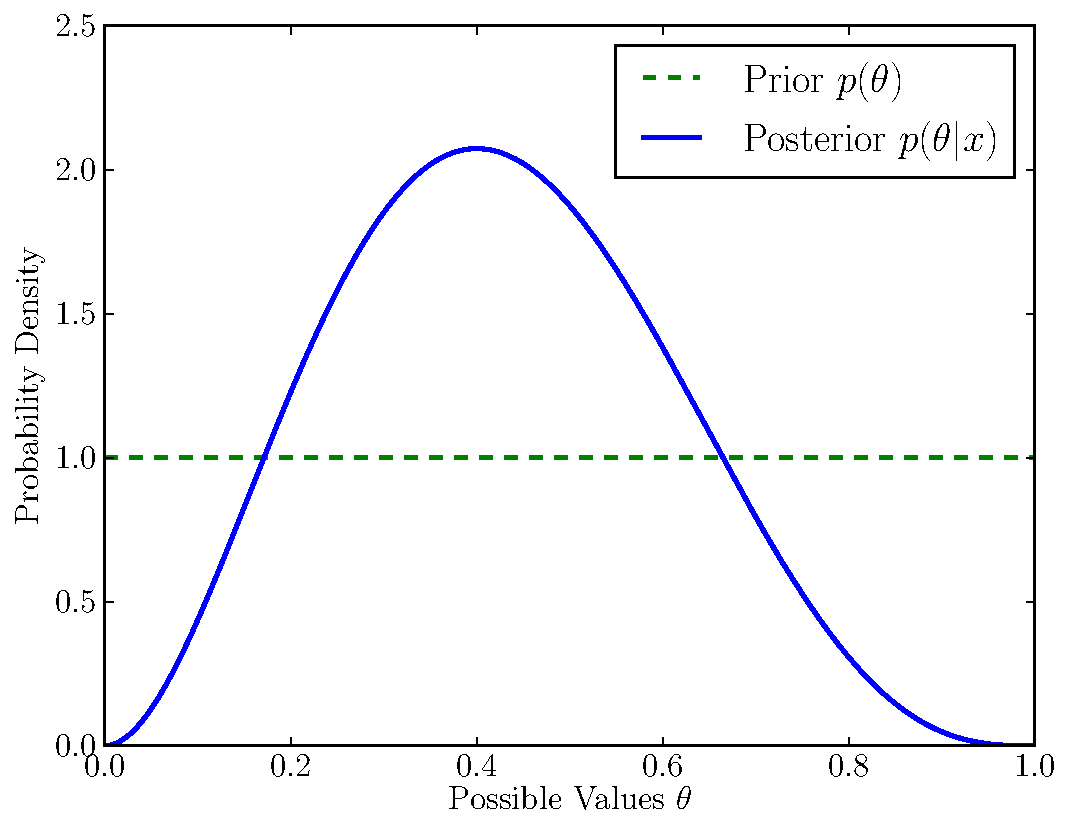
\includegraphics[scale=0.6]{Figures/bus_inference.pdf}
\caption{\it The prior and the posterior for $\theta$ in the bus problem, given
that we had 2/5 successes. The prior is just a uniform density and this is
plotted as a flat line, describing the fact that $\theta$ can be anywhere between
0 and 1 and we don't have much of an idea. After getting the data, the distribution
changes to the posterior which is peaked at 0.4, although there is still a pretty
wide range of uncertainty.\label{fig:bus_inference}}
\end{center}
\end{figure}

\section{``$\sim$'' Notation}
While it is very helpful to know the full equations for different kinds of
probability distributions (both discrete and continuous), it is
useful to be able to communicate about probability distributions in an
easier manner. There is a good notation for this which we will sometimes use
in STATS 331. If we want to communicate about our above analysis, and someone
wanted to know what prior distribution we used, we could do several things.
We could say ``the prior for $\theta$
was uniform between 0 and 1'', or we could give the formula for the prior distribution
(Equation~\ref{eq:uniform}). However, a convenient shorthand in common use is
to simply write:
\begin{eqnarray}
\theta \sim \textnormal{Uniform}(0, 1)
\end{eqnarray}
or, even more concisely:
\begin{eqnarray}
\theta \sim U(0, 1).
\end{eqnarray}
This notation conserves ink, and is good for quick communication.
It is also
very similar to the notation used in JAGS, which will be introduced in later
chapters.

We can also write the binomial likelihood (which we used for the bus problem)
in this notation, instead of writing out
the full equation (Equation~\ref{eq:binomial_likelihood}). We can write:
\begin{eqnarray}
x | \theta \sim \textnormal{Binomial}(N, \theta)
\end{eqnarray}
This says that if we knew the value of $\theta$, $x$ would have a binomial
distribution with $N$ trials and success probability $\theta$. We can also
make this one more concise:
\begin{eqnarray}
x \sim \textnormal{Bin}(N, \theta)
\end{eqnarray}
The differences here are that ``Binomial'' has been shortened to ``Bin'' and
the ``given $\theta$'' part has been left out. However, we see that there is
a $\theta$ present on the right hand side, so the ``given $\theta$'' must
be understood implicitly.

\section{The Effect of Different Priors}
We decided to do this problem with a uniform prior, because it is the obvious
first choice to describe ``prior ignorance''. However, in principle, the prior
could be different. This will change the posterior distribution, and hence
the conclusions. This isn't a problem of Bayesian analysis, but a feature. Data
on its own doesn't tell us exactly what should believe. We must
combine the data with all our other prior knowledge (i.e. put the data in context)
to arrive at reasoned conclusions.

In this section we will look at the effect of different priors
on the results, again focusing on the bus problem for continuity.
Specifically, we will look at three different priors: the
uniform one that we already used, and two other priors discussed below.

\subsection{Prior 2: Emphasising the Extremes}
One possible criticism of the uniform prior is that there is not much probability
given to extreme solutions. For example, according to the Uniform(0, 1) prior,
the prior probability that $\theta$ is
between 0 and 0.1 is only $\int_0^{0.1} 1 \, d\theta = 0.1$. But, depending on the situation, we might think
values near zero should be more plausible\footnote{Here's another parameter that is between 0 and 1: the proportion of
households in New Zealand that keep a Macaw as a pet (call that $\phi$).
I hope this number is low
(it is very difficult to take responsible care of such a smart bird). I also
think it probably is low. I would definitely object to a prior that implied
$P(\phi < 0.1) = 0.1$. I would want a prior that implied something like
$P(\phi < 0.1) = 0.999999$.}.
One
possible choice of prior distribution
that assigns more probability to the extreme values (close to 0 or 1) is:
\begin{eqnarray}
p(\theta) \propto \theta^{-\frac{1}{2}}(1 - \theta)^{-\frac{1}{2}}.\label{eq:prior2}
\end{eqnarray}

\subsection{Prior 3: Already Being Well Informed}
Here's another scenario that we might want to describe in our prior.
Suppose that, before getting this data, you weren't ignorant at all, but already
had a lot of information about the value of the parameter. Say that we already had a lot of information which
suggested the value of $\theta$ was probably close to 0.5. This could be modelled
by the following choice of prior:
\begin{eqnarray}
p(\theta) \propto \theta^{100}(1 - \theta)^{100}.\label{eq:prior3}
\end{eqnarray}

The three priors are plotted in Figure~\ref{fig:three_priors} as dotted lines.
The three corresponding posterior distributions are plotted as solid lines.
The posteriors were computed by multiplying the three priors by the likelihood
and normalising.
The blue curves correspond to the uniform prior we used before, the red
curves use the ``emphasising the extremes'' prior, and the green curves use the
``informative'' prior which assumes that $\theta$ is known to be close to 0.5.

\begin{figure}[h!]
\begin{center}
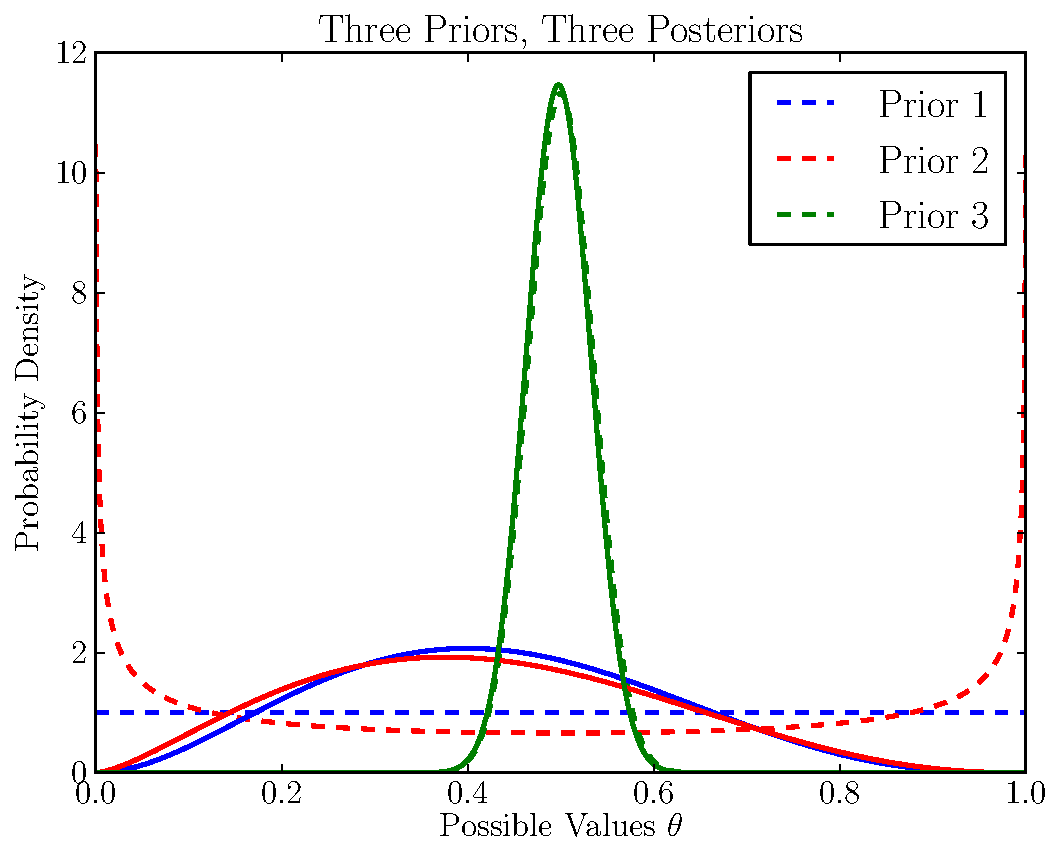
\includegraphics[scale=0.6]{Figures/three_priors.pdf}
\caption{\it Three different priors (dotted lines) and the corresponding
three posteriors (solid lines) given the bus example data. See the text
for discussion of these results.\label{fig:three_priors}}
\end{center}
\end{figure}

There are a few interesting things to notice about this plot. Firstly, the
posterior distributions are basically the same for the red and blue priors (the
uniform prior and the ``emphasising the extremes'' prior). The main difference in the
posterior is, as you would expect, that the extremes are emphasised a little
more. If something is more plausible before you get the data, it's more
plausible afterwards as well.

The big difference is with the informative prior. Here, we were already pretty
confident that $\theta$ was close to 0.5, and the data (since it's not very
much data) hasn't given us any reason to doubt that, so we still think $\theta$
is close to 0.5. Since we already knew that $\theta$ was close to 0.5, the data
are acting only to increase the precision of our estimate (i.e. make the
posterior distribution narrower). But since we had so much prior information,
the data aren't providing much ``extra'' information, and the posterior looks
basically the same as the prior.

\subsection{The Beta Distribution}
The three priors we have used are all examples of {\it beta} distributions. The beta
distributions are a family of probability distributions (like the normal, Poisson,
binomial, and so on) which can be applied to continuous random variables known
to be between 0 and 1. The general form of a beta distribution (here written
for a variable $x$) is:
\begin{eqnarray}
p(x|\alpha, \beta) \propto x^{\alpha - 1}(1 - x)^{\beta - 1}\label{eq:beta}.
\end{eqnarray}
The quantities $\alpha$ and $\beta$ are two parameters that control the shape
of the beta distribution. Since we know the variable $x$ is between 0 and 1 with probability 1, the
normalisation constant could be found by doing an integral. Then you could write
the probability distribution with an equals sign instead of a proportional sign,
\begin{eqnarray}
p(x|\alpha, \beta) &=& \frac{x^{\alpha - 1}(1 - x)^{\beta - 1}}
{\int_0^1 x^{\alpha - 1}(1 - x)^{\beta - 1} \, dx}\\
&=& \frac{x^{\alpha - 1}(1 - x)^{\beta - 1}}
{B(\alpha, \beta)}.
\end{eqnarray}
where $B(\alpha, \beta)$ (called the ``beta function'') is defined (usefully\ldots) as the
result of doing that very integral (it can be related to factorials too, if you're interested).
Thankfully, we can get away with the ``proportional'' version most of the time.
In ``$\sim$'' notation the beta distribution is written as:
\begin{eqnarray}
x|\alpha, \beta &\sim& \textnormal{Beta}(\alpha, \beta).
\end{eqnarray}
Again, the ``given $\alpha$ and $\beta$'' can be dropped. It is implicit because
they appear on the right hand side. By identifying the terms of
Equation~\ref{eq:beta} with the form of our three priors (Equations~\ref{eq:uniform},~\ref{eq:prior2} and~\ref{eq:prior3})),
we see that our three priors can be written in ``$\sim$'' notation like this:

\begin{table}[ht!]\begin{center}
\begin{tabular}{ll}
Prior 1: & $\theta \sim \textnormal{Beta}(1, 1)$\\
Prior 2: & $\theta \sim \textnormal{Beta}\left(\frac{1}{2}, \frac{1}{2}\right)$\\
Prior 3: & $\theta \sim \textnormal{Beta}(101, 101)$\\
\end{tabular}\end{center}
\end{table}

When you work out the posterior distributions analytically and then compare them
to the formula for the beta distribution, you can see that the three posteriors
are also beta distributions! Specifically, you get:

\begin{table}[ht!]\begin{center}
\begin{tabular}{ll}
Posterior 1: & $\theta \sim \textnormal{Beta}(3, 4)$\\
Posterior 2: & $\theta \sim \textnormal{Beta}(2.5, 3.5)$\\
Posterior 3: & $\theta \sim \textnormal{Beta}(103, 104)$
\end{tabular}\end{center}
\end{table}
This is ``magic'' that is made possible by the mathematical form of the beta
prior and the binomial likelihood\footnote{The technical term for this magic is ``conjugate priors''.}. It is not always possible to do this.

Remember that in this particular problem, the probability of a success tomorrow
is simply the expectation value (mean) of the posterior distribution for $\theta$.
We can look up (or derive) the formula for the mean of a beta distribution and find that
if $x \sim \textnormal{Beta}(\alpha, \beta)$ then $\mathds{E}(x) = \alpha/(\alpha + \beta)$.
Applying this to the three posterior distributions gives:

\begin{table}[ht!]\begin{center}
\begin{tabular}{lll}
$P(\textnormal{good bus tomorrow}|x) = 3/7 $    & $\approx 0.429$ & (using prior 1)\\
$P(\textnormal{good bus tomorrow}|x) = 2.5/6$   & $\approx 0.417$ & (using prior 2)\\
$P(\textnormal{good bus tomorrow}|x) = 103/207$ & $\approx 0.498$ & (using prior 3)
\end{tabular}\end{center}
\end{table}
The result for Prior 1 is Laplace's infamous ``rule of succession'' which I will
discuss a little bit in lectures.

\subsection{A Lot of Data}
As shown above, the choice of prior distribution has an impact on the conclusions. Sometimes
it has a big impact (the results using prior 3 were pretty different to the results
from priors 1 and 2), and sometimes not much impact (e.g. the results from
priors 1 and 2 were pretty similar). There is a common phenomenon that happens
when there is a lot of data: the prior tends not to matter so much. Imagine
we did a much bigger version of the bus experiment with $N=1000$ trials, which
resulted in $x=500$ successes. Then the posterior distributions corresponding
to the three different priors are all very similar (Figure~\ref{fig:lots_of_data}).

\begin{figure}[ht!]
\begin{center}
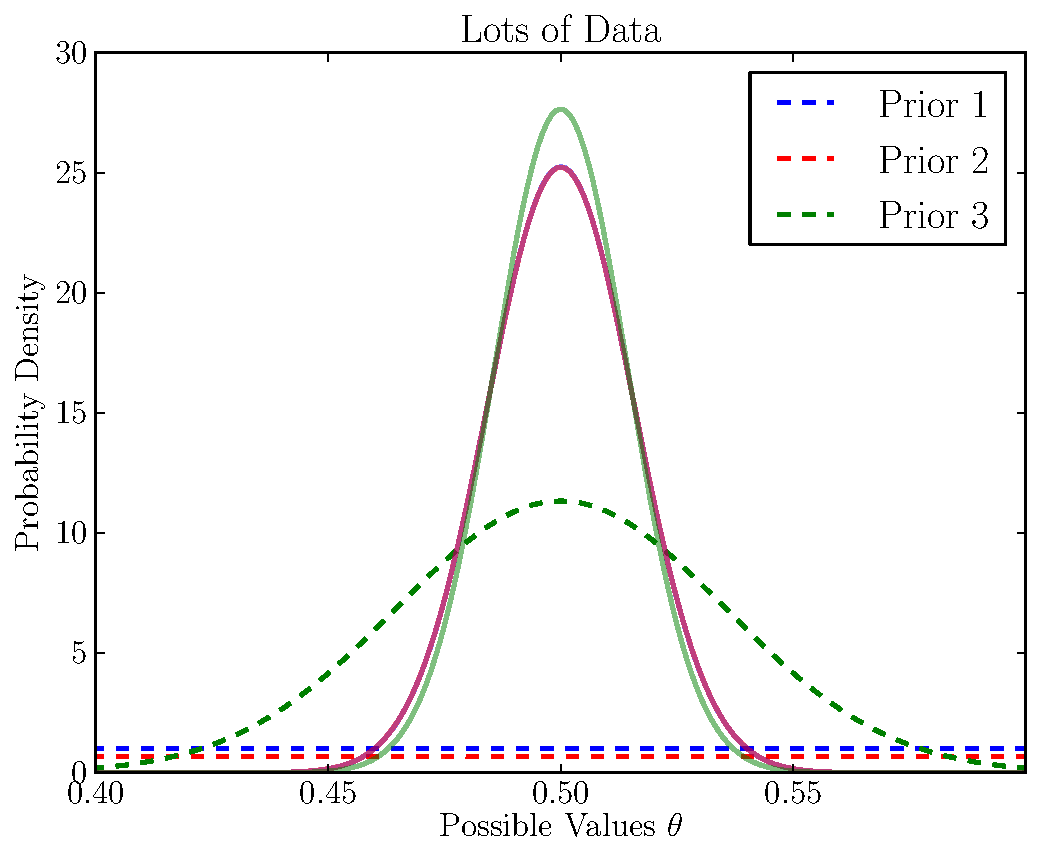
\includegraphics[scale=0.6]{Figures/lots_of_data.pdf}
\caption{\it When you have a lot of data, the results are less sensitive
to the choice of prior distribution. Note that we have zoomed in and are only
looking around $\theta=0.5$: these posterior distributions are quite narrow
because there is now a lot more information about $\theta$. The red and blue
posteriors (based on priors 1 and 2) are so similar that they overlap and look
like one purple curve.\label{fig:lots_of_data}}
\end{center}
\end{figure}

This is reassuring. Note, however, that this only occurs because the three
analyses used the same likelihood. If three people have different prior
distributions for something {\it and} they can't agree on what the experiment
even means, there is no guarantee they will end up agreeing!

Remember though, that when the results {\it are} sensitive
to the choice of prior, that is not a problem with the Bayesian approach, but
rather an important warning message: the data aren't very
informative! Then, the options are: i) think really hard about your prior
distribution and be careful when deciding what it should be, and ii) get more or
better data!

